\section{Validation et performances}

PlaFRIM n'a pas été fonctionnel pendant les vacances, période où nous n'avions pas fini le projet. Cette section propose de présenter le processus de validation, et les résultats obtenus.

\subsection{Validité}

Plusieurs points sont à valider dans le programme : notamment le bon fonctionnement de l'automate de communication et du vol de tâche. La validation de l'automate et des actions associées (menant au vol de tâche) est un processus complexe mettant en jeu des verrous et des sémaphores, aucune validation formelle n'est donc faîte, cela serait possible, mais n'entre pas dans le cadre de notre formation.

En pratique, nous vérifions que des \emph{deadlocks} (entre autres problèmes possibles : communication bloquée, attente active ne terminant pas ...) ne se produisent pas uniquement en considérant que le programme parallèle doit mettre moins de temps que le programme séquentiel. Des messages peuvent être affichés pour informer l'utilisateur de vols de tâches, et de l'avancement du programme général. Ils sont actuellement commentés dans le code, pour ne pas trop ralentir l'exécution pendant les tests (et aussi ne pas surcharger l'affichage).

Enfin pour vérifier que l'image est bien formée, nous avons enregistré un témoin (réalisé séquentiellement) et nous nous contentons de vérifier visuellement la correspondance de notre résultat avec le témoin.

\subsection{\emph{benchmarks}}

Il aurait été intéressant de produire des courbes de performances du type : temps d'exécution en fonction du nombre de processus, ou encore temps d'exécution en fonction de la taille des tuiles, ou enfin temps d'exécution en fonction du nombre de \emph{threads} par processus. Pour toutes ces fonctions, il existe probablement à chaque fois une valeur optimale (nombre de processus, \emph{threads} ou \emph{pixels} par tuile) qui donnerait à ces courbes une forme de cloche inversée.

Les raisons à une remontée du temps d'exécution pour toutes ces fonctions lorsque l'on rajoute des ressources sont : 
\begin{itemize}
\item[$\bullet$] temps de communications en anneau prohibitifs si trop de processus ;
\item[$\bullet$] équivalence avec le programme séquentiel si les tuiles font la taille de l'image, ou inversement utilisation intensive (et donc bloquante) des verrous si les tuiles correspondent à un seul \emph{pixel} ;
\item[$\bullet$] dépassement mémoire et utilisation trop intensive des verrous si trop de \emph{threads}.
\end{itemize}

La version jouet du programme n'a pas été implémentée, elle aurait cependant permis de créer des cas probants de vol de tâches. Une idée simple étant d'associer le temps d'exécution d'une tâche à un multiple du rang du processus qui l'a créée, ainsi le processus $0$ finira beaucoup plus tôt (instantanément ...) que les autres, et volera des tâches au processus $1$ qui lui aussi est censé terminer beaucoup plus tôt que le $2$, etc ...\\
Un script a été écrit afin de créer automatiquement la première courbe : le temps d'exécution en fonction du nombre de processus. Le graphe a été dessiné pour les trois implémentations du \emph{thread} de communication présentées dans la section précédente. Le nombre de processus utilisés varie entre $1$ et $32$, en pratique il s'agit de \texttt{qsub} fait avec $1$ n\oe ud avec $1$ c\oe ur, puis $1$ n\oe ud avec $2$ c\oe urs \ldots $4$ n\oe uds avec $8$ c\oe urs. Il y a donc une différence de répartition entre $15$ et $16$ processus : le premier utilise $3$ n\oe uds tandis que le second en utilise $4$.
\begin{itemize}
\item[$\bullet$] Première version : figure \ref{img:graph1}. Ce graphe a été tracé quand, par chance, aucun \emph{deadlock} ne se produisait. La principale chose à remarquer est la présence de pics du temps d'exécution, pour $9$ processus, $16$, $20$ et $24$. Ceux-ci sont dûs aux changements du nombre de n\oe uds utilisés par rapport au nombre de processus supérieur et inférieur. Ainsi $20 = 4_{noeuds} \times 5_{coeurs}$ est compris entre $18 = 3_{noeuds} \times 6_{coeurs}$ et $21 = 3_{noeuds} \times 7_{coeurs}$. Ces pics sont la traduction du fait que les communications sont plus lentes lorsqu'elles nécessitent plus de n\oe uds différents.
\item[$\bullet$] Seconde version : figure \ref{img:graph2}. Sur ce graphe, les pics sont moins élevés. En effet la terminaison qui nécessite normalement beaucoup de communications se fait ici par une sorte de \emph{broadcast} (en réalité il s'agit de plusieurs envois réalisés à la suite) de la racine vers les autres processus, moins de communications passent donc par l'anneau de communication, la terminaison est plus rapide. La scalabilité du programme, du fait de la faiblesse des pics est ici mieux visible : le temps d'exécution est faible au milieu, et atteint une valeur optimale (i. e. minimale) pour $6$ et $8$ processus. Pour un nombre élevé de processus $28$ ou pour un nombre faible $1$, la scalabilité est inexistante, le temps d'exécution est alors $50 \%$ supérieur au temps optimal. La courbe est typique d'un programme parallèle, plus ou moins en cloche inversée.
\item[$\bullet$] Troisième version : figure \ref{img:graph3}. Même remarques que pour la première version, avec toutefois un temps d'exécution globalement plus rapide (car compilé avec \texttt{-02}).
\end{itemize}


\begin{figure}
\raggedright
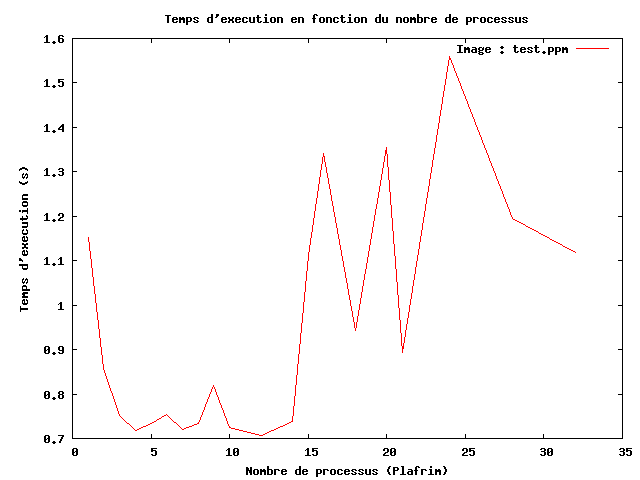
\includegraphics[scale=0.5]{dead_graph_procs.png}
\caption{Première implémentation.}
\label{img:graph1}
\end{figure}

\begin{figure}
\raggedright
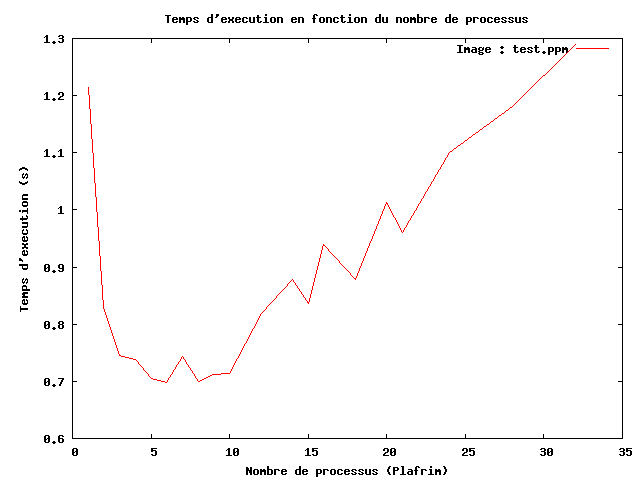
\includegraphics[scale=0.5]{for_graph_procs.png}
\caption{Seconde implémentation.}
\label{img:graph2}
\end{figure}

\begin{figure}
\raggedright
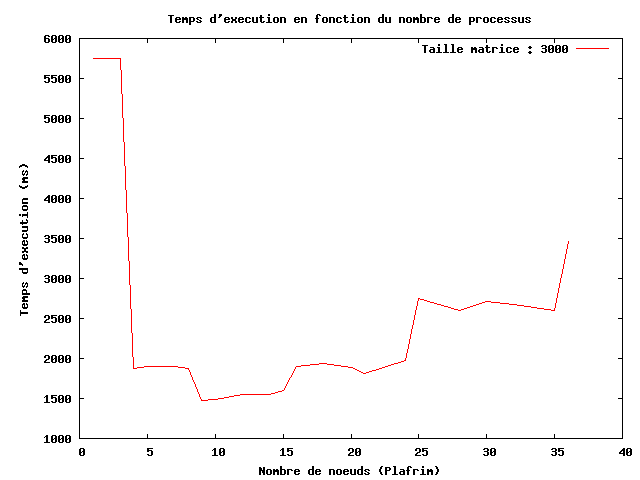
\includegraphics[scale=0.5]{graph_procs.png}
\caption{Troisième implémentation.}
\label{img:graph3}
\end{figure}
